\documentclass[aspectratio=169]{beamer}
\usetheme{Singapore}

% add page numbers at the bottom of the slides
\setbeamertemplate{caption}[numbered]
\addtobeamertemplate{navigation symbols}{}{%
    \usebeamerfont{footline}%
    \usebeamercolor[fg]{footline}%
    \hspace{1em}%
    \raisebox{1.4pt}[0pt][0pt]{\insertframenumber/\inserttotalframenumber}
}

% \definecolor{primarycolor}{HTML}{0000FF}

% \makeatletter

% \def\sectioncolor{primarycolor}% color to be applied to section headers

% \setbeamercolor{palette primary}{use=structure,fg=structure.fg}
% \setbeamercolor{palette secondary}{use=structure,fg=structure.fg!75!black}
% \setbeamercolor{palette tertiary}{use=structure,fg=structure.fg!50!black}
% \setbeamercolor{palette quaternary}{fg=black}

% \setbeamercolor{local structure}{fg=primarycolor}
% \setbeamercolor{structure}{fg=primarycolor}
% \setbeamercolor{title}{fg=primarycolor}
% \setbeamercolor{section in head/foot}{fg=black}

% \setbeamercolor{normal text}{fg=black,bg=white}
% \setbeamercolor{block title alerted}{fg=red}
% \setbeamercolor{block title example}{fg=primarycolor}

% \setbeamercolor{footline}{fg=primarycolor!50}
% \setbeamerfont{footline}{series=\bfseries}

% use classic LaTeX font for maths
\usefonttheme[onlymath]{serif}

\usepackage{cmap}
\usepackage[english]{babel}
\usepackage[T1]{fontenc}
\usepackage[utf8]{inputenc}
\usepackage[kerning=true]{microtype}
\usepackage{lmodern}

\usepackage{amsmath}
\usepackage{amsfonts}
\usepackage{amssymb}
\usepackage{amsthm}

\usepackage{mathtools}
\usepackage{wrapfig}
\usepackage{enumitem}
\usepackage{tikz}
\usepackage{xcolor}
\usetikzlibrary{positioning}

\usepackage[
    backend=biber,
    style=numeric,
]{biblatex}
\usepackage{graphicx}
\usepackage[justification=centering]{caption}
\usepackage{csquotes}

\graphicspath{{./images/}}

\addbibresource{../report/report.bib}
% \renewcommand*{\bibfont}{\footnotesize}

\AtBeginSection[]
{
  \begin{frame}
    \frametitle{Plan}
    \tableofcontents[currentsection]
  \end{frame}
}


\theoremstyle{definition}
\newtheorem*{exemple}{Example}

\renewcommand{\leq}{\leqslant}
\renewcommand{\geq}{\geqslant}

\setbeamertemplate{itemize items}[circle]


\title{\textbf{Implementation of an\\Iterative Linear Quadratic Regulator (iLQR)}}
\author{Gabriel Desfrene\and Antoine Groudiev}

\titlegraphic{
\includegraphics[height=1.8cm]{./images/logo-ens-psl.png}}

\date{January 14, 2025}

\begin{document}
\frame{\titlepage}

\begin{frame}{Plan}
   \tableofcontents
\end{frame}

\section{Problem statement}
\begin{frame}{General formulation}
    \begin{itemize}
        \item Dynamics function:
        \begin{equation*}
            x_{t+1} = f(x_t, u_t)
        \end{equation*}
        \item Goal: minimize a quadratic cost function
        \item Cost function:
        \begin{equation*}
            J(u) = \sum_{t=0}^{T-1} \left(x_t^\top Q x_t + u_t^\top R u_t\right) + \frac{1}{2}(x_T-x^*)^\top Q_f (x_T-x^*)
        \end{equation*}
        \item $Q$: state cost matrix
        \item $Q_f$: final state cost matrix
        \item $R$: control cost matrix
    \end{itemize}
\end{frame}

\begin{frame}{Example: Simple Pendulum}
    \begin{minipage}[c]{0.6\linewidth}
        \begin{itemize}
            \item State: $x = [\theta\:\:\:\dot{\theta}]$
            \item Control: $u$, torque applied to the pendulum
            \item Dynamics: physical laws (simulator)
            \item Target: $x=[0\:\:\:0]$
            \item Cost function:
            \begin{equation*}
                J(u) = \frac{1}{2}\left(\theta_f^2+\dot{\theta}_f^2\right) + \frac{1}{2}\int_0^T ru^2(t) \mathrm{d} t
            \end{equation*}
            corresponding to $Q_f = I_2$, $Q=0_2$, $R=rI_1$
        \end{itemize}
    \end{minipage}
    \hspace{0.25cm}
    \begin{minipage}[c]{0.35\linewidth}
        \begin{figure}
            \centering
            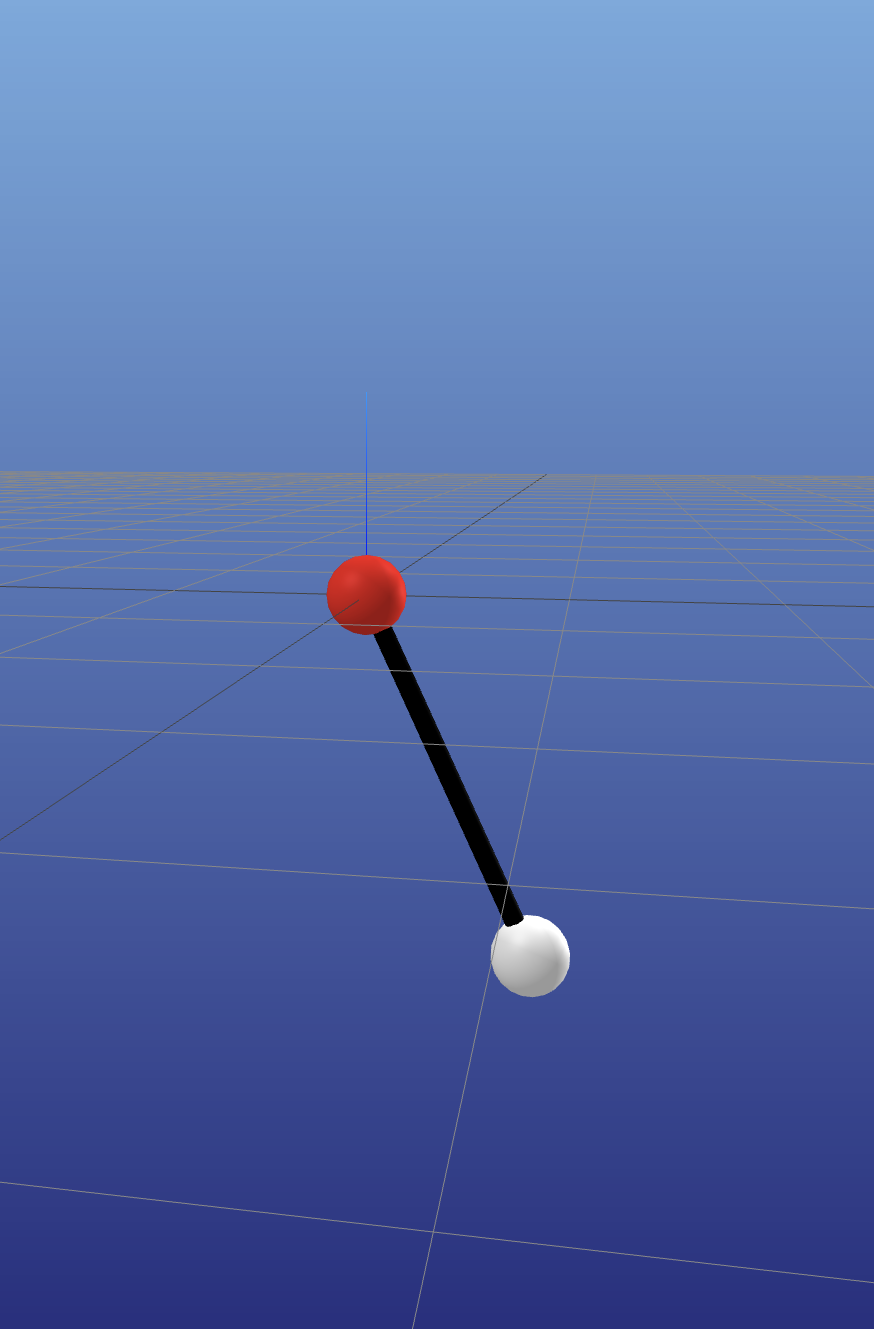
\includegraphics[width=0.7\linewidth]{pendulum.png}
        \end{figure}
    \end{minipage}
\end{frame}

\begin{frame}{Example: Cartpole}
    \begin{minipage}[c]{0.6\linewidth}
        \begin{itemize}
            \item State: $x=[y\:\:\:\theta\:\:\:\dot{y}\:\:\:\dot{\theta}]$
            \item Control: $u$, force applied to the cart
            \item Dynamics: physical laws (simulator)
            \item Target: $x=[0\:\:\:0\:\:\:0\:\:\:0]$
            \item Cost function:
            \begin{equation*}
                J(u) = \frac{1}{2}\left(\theta_f^2+\dot{\theta}_f^2 + y_f^2 + \dot{y}_f^2\right) + \frac{1}{2}\int_0^T ru^2(t) \mathrm{d} t
            \end{equation*}
            corresponding to $Q_f = I_4$, $Q=0_4$, $R=rI_1$
        \end{itemize}
    \end{minipage}
    \hspace{0.25cm}
    \begin{minipage}[c]{0.35\linewidth}
        \begin{figure}
            \centering
            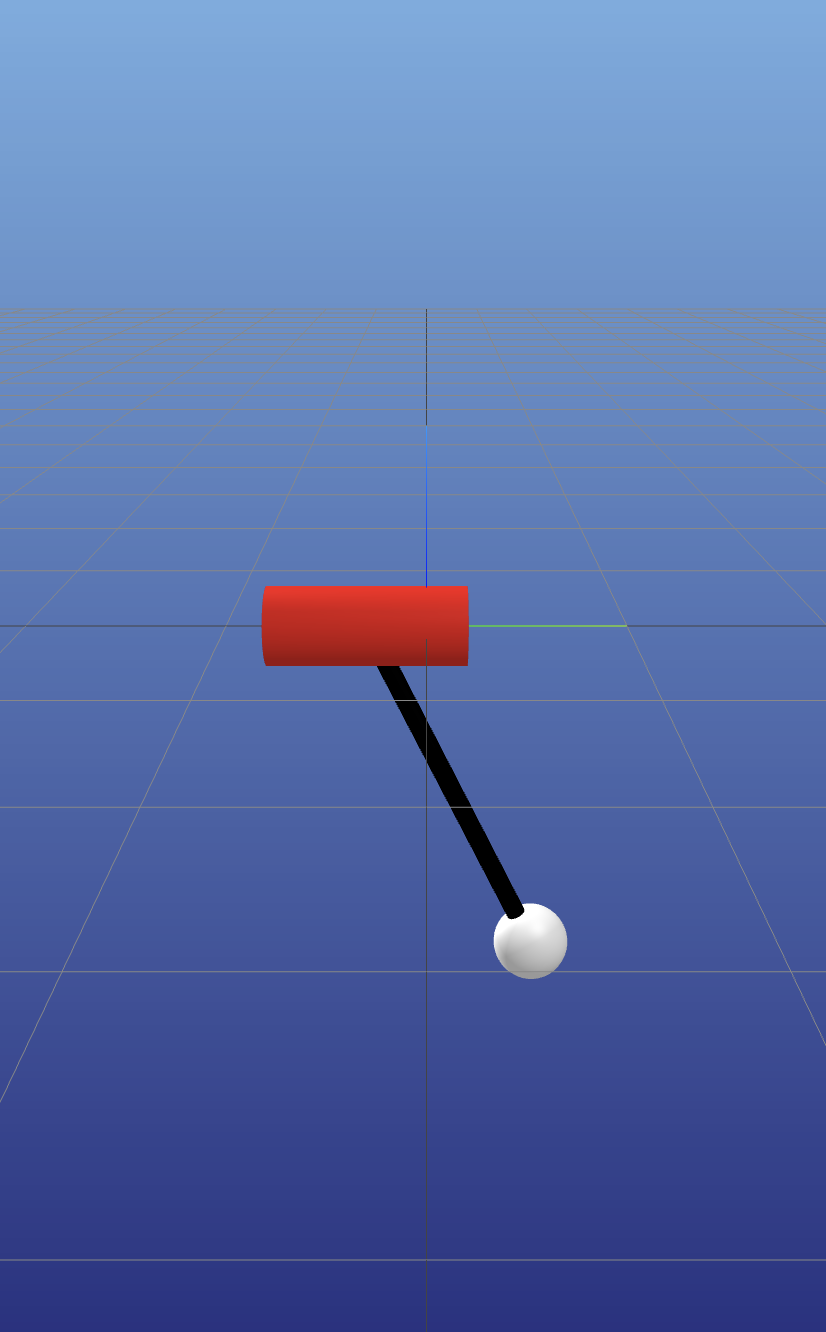
\includegraphics[width=0.7\linewidth]{cartpole.png}
        \end{figure}
    \end{minipage}
\end{frame}

\section{The iLQR algorithm}


\begin{frame}[allowframebreaks]
    \nocite{*}
    \printbibliography
\end{frame}

\end{document}